\documentclass[UTF8, 12pt]{ctexart}

\usepackage{amsmath}

\usepackage{geometry}
\geometry{a4paper, scale = 0.9} % a4纸, 版心占页面长度的比例为0.9

\usepackage{enumitem} % itemize, 列表

\usepackage{graphicx}

\begin{document}

	\noindent
	整流电路 :

	单相半波整流电路 :

	电路图 :

	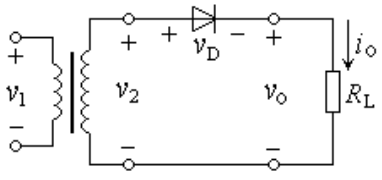
\includegraphics[scale = 0.4]{08/单相半波整流电路电路图.png}

	分析 :
	\begin{itemize}[leftmargin = 4em]
		\item 正半周期二极管导通, 负半周期二极管截止
		\item 输出电压平均值 $ \frac{\sqrt{2}}{\pi}V_{2} $
		\item 脉动系数(输出电压基波最大值和平均值之比) $ \frac{\pi}{2} $
	\end{itemize}

	单相桥式整流电路 :

	电路图 :

	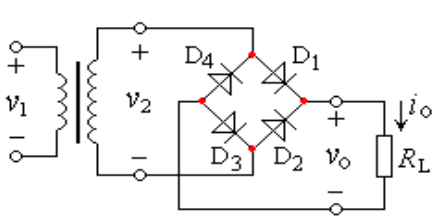
\includegraphics[scale = 0.4]{08/单相桥式整流电路电路图.png}

	分析 :
	\begin{itemize}[leftmargin = 4em]
		\item 正半周期 $ D_{1}, D_{3} $ 导通, 负半周期$ D_{2}, D_{4} $ 导通
		\item 输出电压平均值 $ \frac{2\sqrt{2}}{\pi}V_{2} $
		\item 脉动系数 $ \frac{2}{3} $
	\end{itemize}

	电容滤波电路 :

	电路图 :

	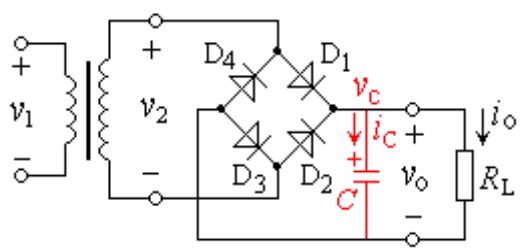
\includegraphics[scale = 0.4]{08/电容滤波电路电路图.png}

	分析 :
	\begin{itemize}[leftmargin = 4em]
		\item 空载 : $ u_{2} > u_{c} $ 电容充电, $ u_{2} < u_{c} $ 电容保持(无放电电路)
		\item 负载(RC较大) : 放电慢充电快, 电压平均值大, 脉动成分降低
	\end{itemize}

	~

	\noindent
	稳压电路 :
	
	稳压管稳压电路 :

	电路图 :

	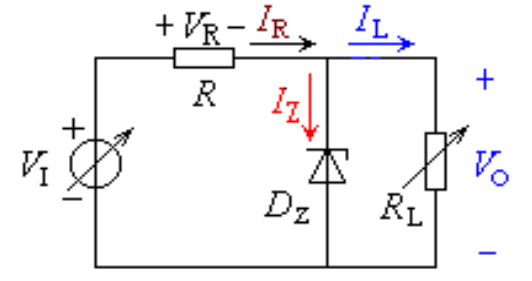
\includegraphics[scale = 0.4]{08/稳压管稳压电路电路图.png}

	串联型稳压电路 :

	电路图 :

	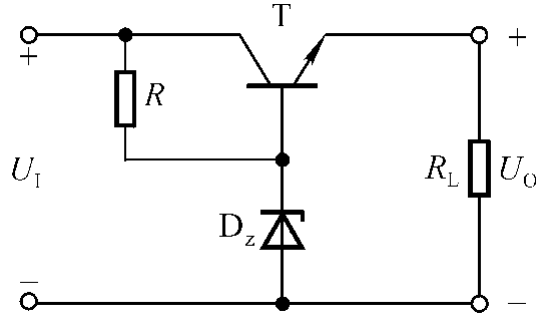
\includegraphics[scale = 0.4]{08/串联型稳压电路.png}

\end{document}